\providecommand{\main}{../..}
\documentclass[\main/notes.tex]{subfiles}

\begin{document}
	\setcounter{chapter}{4}
	\chapter{Organising and Storing Data}
		\section{Data Management and Data Modelling}
			\begin{definition}{Relational Database}
				A series of related tables, stored together with a minimum of duplication to achieve a consistent and controlled pool of data.
			\end{definition}
			\begin{definition}{Entity}
				A person, place, or thing about whom or about which an organisation wants to store data.
			\end{definition}
			\begin{definition}{Record}
				A row in a table; all the data pertaining to one instance of an entity.
			\end{definition}
			\begin{definition}{Field}
				A characteristic or attribute of an entity that is stored in the database.
			\end{definition}
			\begin{definition}{Primary Key}
				A field in a table that is unique -- each record in that table has a different value in the primary key field. Used to uniquely identify each record and to create relationships between tables.
			\end{definition}
			\begin{sidenote}{Advantages of the Database Approach}
				\begin{multicols}{2}
					\begin{itemize}[nosep]
						\item Improved strategic use of corporate data
						\item Reduced data redundancy
						\item Easier modification and updating
						\item Data and program independence
						\item Better access to data and information
						\item Standardisation of data access
						\item A framework for program development
						\item Better overall protection of the data
						\item Shared data and information resources
					\end{itemize}
				\end{multicols}
			\end{sidenote}
			\begin{sidenote}{Disadvantages of the Database Approach}
				\begin{multicols}{2}
					\begin{itemize}
						\item More complexity
						\item More difficult to recover from a failure
						\item More expensive
					\end{itemize}
				\end{multicols}
			\end{sidenote}
			\subsection{Relationships Between Tables}
				Use a primary key from another table to make the tables related.
				\begin{definition}{Foreign Key}
					When a primary key is posted into another table to create a relationship between the two.
				\end{definition}
			\subsection{Designing Relational Databases}
				\begin{enumerate}[nosep]
					\item Identify all entities
					\item Identify all relationships between entities
					\item Identify all attributes
					\item Resolve all relationships
				\end{enumerate}
				\subsubsection{Identify Entities}
					Determine which entities information needs to be stored about. Usually done by interviewing the firm's managers and staff, or using questionnaires.
				\subsubsection{Identify Relationships}
					Determine what relevant relationships exist between entities. These need to be the relationships the firm wants to store data about.
					\begin{definition}{Degree}
						The number of entities involved in a relationship.
					\end{definition}
					\begin{definition}{Cardinality}
						Whether each entity in a relationship is related to one or more than one of the other entities. The number of one entity that can be related to another entity. Cardinality for a binary relationship can be one to one (1:1), one to many (1:M), or many to many (M:M).
					\end{definition}
					\begin{definition}{Optionality}
						Documents whether a relationship must exist for each entity, or whether it is optional. If a binary relationship is optional for an entity, that entity doesn't have to be related to the other.
					\end{definition}
					\begin{sidenote}{Entity-Relationship Diagram Example}
						\begin{center}
							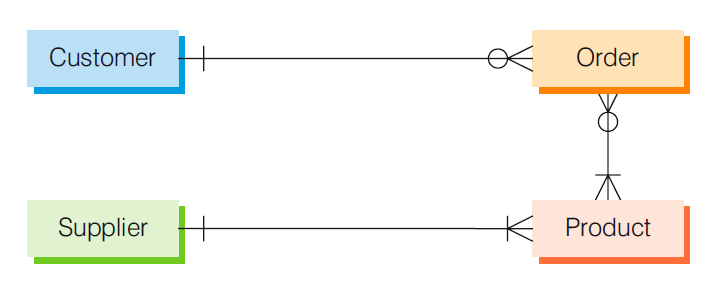
\includegraphics[width=0.85\textwidth]{chapter05/entity_relationship_diagram.png}
						\end{center}
						The crow's foot notation means many, so a supplier supplies many products, but each product is supplied by only one supplier.

						The O and | represent optionality. An O means the relationship is optional, a | means the relationship is obligatory.
					\end{sidenote}
					\begin{definition}{Enterprise Rules}
						The rules governing relationships between entities.
					\end{definition}
					\begin{example}
						Enterprise rules:
						\begin{itemize}
							\item Each order must be placed by one and only one customer
							\item Each customer can place many orders, but some won't have placed any orders
						\end{itemize}
					\end{example}
				\subsubsection{Identify Attributes}
					Identify what information will be stored about each entity. An \concept{attribute} should be the smallest sensible piece of data that is to be stored.
				\subsubsection{Resolve Relationships}
					Determining how a relationship should be implemented.

		\pagebreak
		\section{Database Management Systems}
			\begin{definition}{Database Management System (DBMS)}
				A group of programs used as an interface between a database and application programs, or between a database and the user.
			\end{definition}
			\subsection{Creating and Modifying the Database}
				\begin{definition}{Data Definition Language}
					A collection of instructions and commands used to define and describe data and relationships in a specific database. An example is \concept{Structured Query Language (SQL)}.
				\end{definition}
				\begin{definition}{Data Dictionary}
					A detailed description of all the data used in the database.

					Describes all the fields in the database, their range of accepted values, the type of data, the amount of storage space needed, and a note of who can access, and who can update.
				\end{definition}
			\subsection{Storing and Retrieving Data}
				A DBMS needs to be an interface between an application program and the database. To do this:
				\begin{itemize}
					\item The application requests data from the DBMS, following a \concept{logical access path (LAP)}.
					\item The DBMS accesses a storage device where the data is stored, following a \concept{physical access path (PAP)}.
				\end{itemize}
				\begin{sidenote}{Problems with Access}
					Two or more people or programs trying to access the same record in a database can be problematic. This is called \concept{concurrency}.
				\end{sidenote}
				\begin{definition}{Concurrency Control}
					A method of dealing with a situation in which two or more people need to access the same record in a database at the same time.
				\end{definition}
			\subsection{Manipulating Data and Generating Reports}
				After a DBMS is installed, it can be used to review reports and obtain important information.
				\begin{definition}{Database Manipulation Language (DML)}
					The commands that are used to manipulate the data in the database. SQL can also be used as one of these.
				\end{definition}
			\subsection{Database Administration}
				\begin{definition}{Database Administrator (DBA)}
					The role of the database administrator is to plan, design, create, operate, secure, monitor, and maintain databases.

					Typically, has a degree in computer science or management information systems, and some on-the-job training. 
				\end{definition}
				\begin{definition}{Data Administrator}
					A non-technical position responsible for defining and implementing consistent principles for a variety of data issues.
				\end{definition}
			\subsection{Selecting a Database Management System}
				The DBA often selects the DBMS for an organisation. Begins by analysing database needs and characteristics.
				\begin{sidenote}{Important Characteristics of Databases}
					\begin{description}
						\item[Database size] The number of records or files in the database
						\item[Database cost] The purchase or lease costs of the database
						\item[Concurrent Users] The number of people who need to use the database at the same time
						\item[Performance] How fast the database is able to update records
						\item[Integration] The ability of the database to be integrated with other applications and databases
						\item[Vendor] The reputation and financial stability of the database vendor 
					\end{description}
				\end{sidenote}
			\subsection{Using Databases with Other Software}
				A DBMS can act as a front-end application or a back-end application.
				\begin{indentparagraph}
					\begin{description}
						\item[Front-end application] An application that directly interacts with people or users.
						\item[Back-end application] An application that interacts with other programs or applications; it only indirectly interacts with people or users.
					\end{description}
				\end{indentparagraph}

		\pagebreak
		\section{Database Applications}
			\begin{definition}{Database Application}
				An application that manipulates the content of a database to produce useful information.

				Common manipulations are searching, filtering, synthesizing and assimilating the data in a database.
			\end{definition}
			\subsection{Linking Databases to the Internet}
				Every e-commerce website uses database technology to dynamically create its web pages. This simplifies the maintenance of the website, as any new information just needs to be stored in the database, to update the website.

				\begin{description}
					\item[Semantic Web] Developing a seamless integration of traditional databases with the Internet. Allows people to access and manipulate a number of traditional databases at the same time through the Internet.
				\end{description}
			\subsection{Big Data Applications}
				\begin{definition}{Big Data}
					Large amounts of unstructured data that are difficult or impossible to capture and analyse using traditional DBMS's.

					Can provide valuable insights to help organisations achieve their goals.

					Special hardware and software is needed. \concept{Apache Hadoop} is an open-source database that can be used to manage large, unstructured datasets in conjunction with relational databases.
				\end{definition}
			\subsection{Data Warehouses}
				\begin{definition}{Data Warehouse}
					A database or collection of databases that holds business information from many sources in the enterprise, covering all aspects of the company's processes, products, and customers.

					Provides business users with a multidimensional view of that data they need to analyse business conditions.
				\end{definition}
			\subsection{Data Mining}
				\begin{definition}{Data Mining}
					The process of analysing data to try to discover patterns and relationships within the data.

					A number of rules and techniques can be used. \concept{Association rules algorithms} are used to find associations between items in the data. The application \concept{Rattle}, used in the programming language \concept{R}, is a powerful data mining tool.
				\end{definition}
				\begin{sidenote}{Common Data-Mining Applications}
					\begin{center}
						\begin{tblr}{colspec={>{\raggedright}X[1] >{\raggedright}X[3]}, row{even}={white}, row{1}={font=\bfseries}}
							Application & Description\\
							\midrule
							Branding and positioning of products and services & Enable the strategist to visualise the different positions of competitors in a given market using performance data on dozens of key features of a product.\\
							Customer churn & Predict current customers who are likely to switch to a competitor.\\
							Direct marketing & Identify prospects most likely to respond to a direct marketing campaign.\\
							Fraud detection & Highlight transactions most likely to be deceptive or illegal.\\
							Market basket analysis & Identify products and services that are most commonly purchased at the same time.\\
							Market segmentation & Group customers based on who they are or what they prefer.\\
							Trend analysis & Analyse how key variables (e.g. sales, spending, promotions) vary over time.
						\end{tblr}
					\end{center}
				\end{sidenote}
			\subsection{Business Intelligence}
				\begin{definition}{Business Intelligence (BI)}
					The process of gathering enough of the right information in a timely manner and usable form, and analysing it to have a positive impact on business strategy, tactics, or operations. An example of BI software is \concept{Zoho Analytics}.
				\end{definition}
				\begin{definition}{Competitive Intelligence}
					One aspect of business knowledge limited to information about competitors and the ways that knowledge affects strategy, tactics and operations.

					Critical part of a company's ability to see and respond quickly and appropriately to the changing marketplace.

					\emph{Not} espionage: the use of illegal means to gather information.
				\end{definition}
				\begin{definition}{Counterintelligence}
					The steps an organisation takes to protect information sought by `hostile' intelligence gatherers.
				\end{definition}
			\pagebreak
			\subsection{Distributed Databases}
				\begin{definition}{Distributed Database}
					A database in which the data is spread across several smaller databases connected via telecommunications devices.
				\end{definition}
				\subsubsection{Wide Column Store}
					Distributed databases often don't use the relational model. Instead, they use \concept{wide column store}. \emph{Don't} use SQL, called \concept{NoSQL databases}. Can be thought of as a set of tables that don't have the same number of columns in each row.

					More flexibility in the way databases are organised and used, but creates additional challenges in integrating different databases. As they rely on telecommunications, access to data can be slower.
					\begin{definition}{Replicated Database}
						A database that holds a duplicate set of frequently used data.

						The company sends a copy of important data to each distributed processing location. The location then sends the changed data back, to update the main database on an update cycle. This is called \concept{data synchronisation}.
					\end{definition}
			\subsection{Online Analytical Processing}
				\begin{definition}{Online Analytical Processing (OLAP)}
					Software hat allows users to explore data from a number of perspectives.
				\end{definition}
				\begin{sidenote}{Comparison of OLAP and Data Mining}
					\begin{tblr}{colspec={>{\raggedright}X>{\raggedright}X>{\raggedright}X}, row{even}={white}, row{1}={font=\bfseries}, column{1}={font=\bfseries}}
						Characteristic & OLAP & Data Mining\\
						\midrule
						Purpose & Support data analysis and decision-making & Support data analysis and decision-making\\
						Type of analysis supported & Top-down, query-driven data analysis & Bottom-up, discovery-driven data analysis\\
						Skills required of user & Must be very knowledgeable of the data and its business context & Must trust in data-mining tools to uncover valid and worthwhile hypotheses.
					\end{tblr}
				\end{sidenote}

	\vbox{\rulechapterend}
\end{document}